\documentclass[14pt, oneside]{ctexart}
\usepackage{tikz}
\usepackage{geometry}                		
\geometry{a4paper, margin=2cm}                   				
\usepackage{graphicx}
\usepackage{amsmath}		
\usepackage{amssymb}


\title{Latex使用指南}
\author{丁保华}


\begin{document}
\maketitle

代码示例:
\linespread{2}
\begin{verbatim*}
#include <iostream>
int main()
{
    std::cout << "Hello, world!"
    << std::endl;
    return 0;
}
\end{verbatim*}

\linespread{1}
\begin{verbatim*}
    for (int i=0; i<4; ++i)
        printf("Number %d\n",i);
\end{verbatim*}


\fbox{\begin{minipage}{15em}%
这是一个垂直盒子的测试。
\footnote{脚注来自minipage。}
\end{minipage}}

%设置字体、字号
\[ a^2 + b^2 = c^2 \]

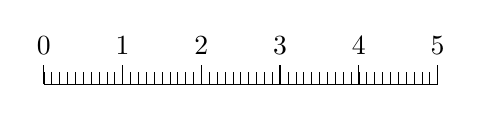
\begin{tikzpicture}
	\draw (0,0)--(5,0);
	\foreach \i in {0.0,0.1,...,5.0}
		{\draw[very thin] (\i,0) --  ++(0,0.15);}
	\foreach \I in {0,1,2,3,4,5}
		{\draw (\I,0) -- ++(0,0.25) node[above] {\I};}
\end{tikzpicture}

\[
E=m \cdot c^2
\]

$\alpha$ is the first letter of Greeks

$\mathbb{Z} \subset \mathbb{R}$

\end{document}  